\section{INTRODUCTION}

Monocular vision comes being a flourishing field in autonomous vehicles. 
Several applications have presented solutions to current problems. 
Although in systems  of low computational cost remain a challenge. 


The Particle Image Velocimetry ($PIV$)\cite{Bastiaans} technique is used in many fields of 
knowledge, \cite{Story, Xu}, to calculate the velocity of fluids in different parts. 
Here, $PIV$ was adjusted for situation of autonomous vehicles, using a matching criteria based on 
the Pearson Correlation Coefficient ($PCC$)\cite{Miranda Neto} over the KITTI dataset\cite{Geiger}.

Here, we define some variables used in the paper. The object that will be subject tracking is defined as target.
A matrix containing only an image of the target is called Region Of Interest ($ROI$).
By other side, a portion of an image that is under analysis is called Window of Search ($WOS$), 
and it is a rectangle where the program will search similarities with the $ROI$.
Finally, each one of sub regions inside the $WOS$ are called analysis region.

\begin{figure}[bhp]
\centering
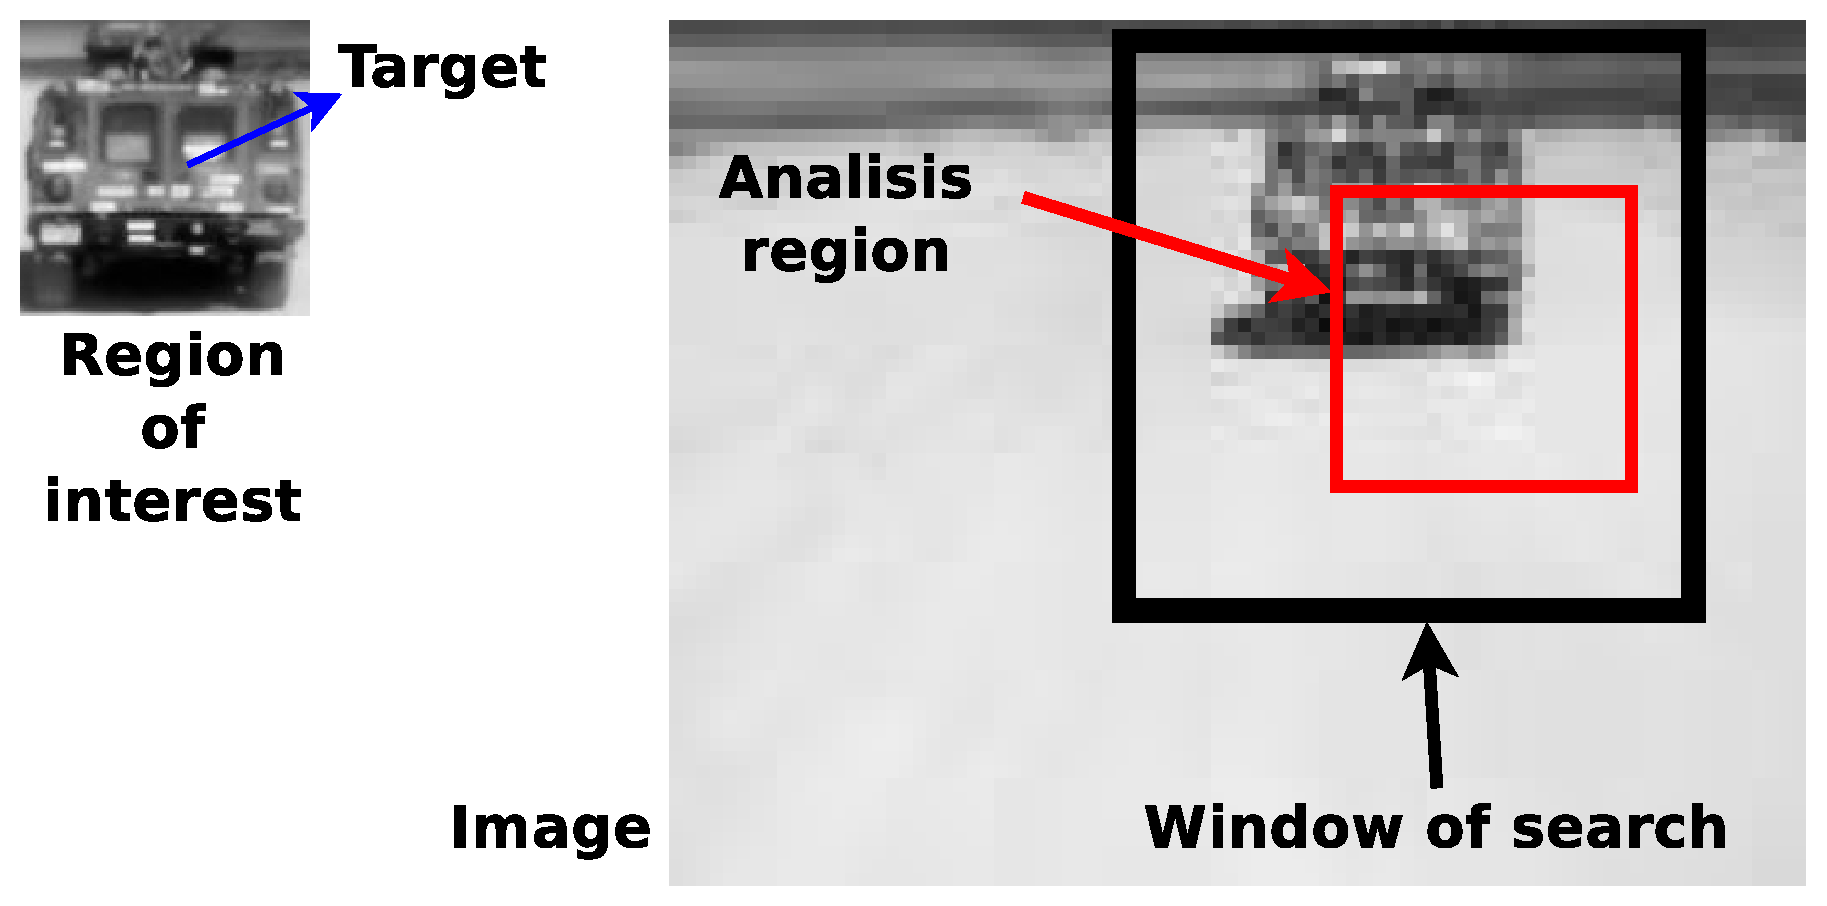
\includegraphics[width=0.7\columnwidth]{images/Diagrama2.eps}
\caption{Notation of variable names used in this paper.}
\label{fig:systemnotation}
\end{figure}

